\documentclass[a4paper, 10pt, final, garamond]{book}
\usepackage{cours-preambule}
\usepackage[french]{babel}

\raggedbottom

\makeatletter
\renewcommand{\@chapapp}{Induction -- chapitres}
\renewcommand\thechapter{1 et 2}
\makeatother

\begin{document}
% \setcounter{chapter}{2}

\chapter{Correction du TD}

\section{Aimant en U}
\label{sec:exaimu}
\noindent
\begin{minipage}[t]{.5\linewidth}
  Voir Figure~\ref{fig:exaimucorr}. Les LdC sortent par le Nord, entrent par le
  Sud. Le champ est fort là où les LdC sont serrées, faible là où elles sont
  éloignées. Il est uniforme là où les LdC sont parallèles et régulièrement
  espacées. Dans l'entrefer (\textbf{dans le métal}), le champ va du Sud au
  Nord.
  \bigbreak
  On peut créer des champs uniformes dans un solénoïde, et au milieu d'une
  bobine de \textsc{Helmoltz}, constituée de deux bobines plates de même rayon
  $R$ et espacées de $R$, parcourues par la même intensité dans le même sens.
\end{minipage}
\begin{minipage}[t]{.5\linewidth}
  ~
  \vspace*{-10pt}
  \begin{center}
    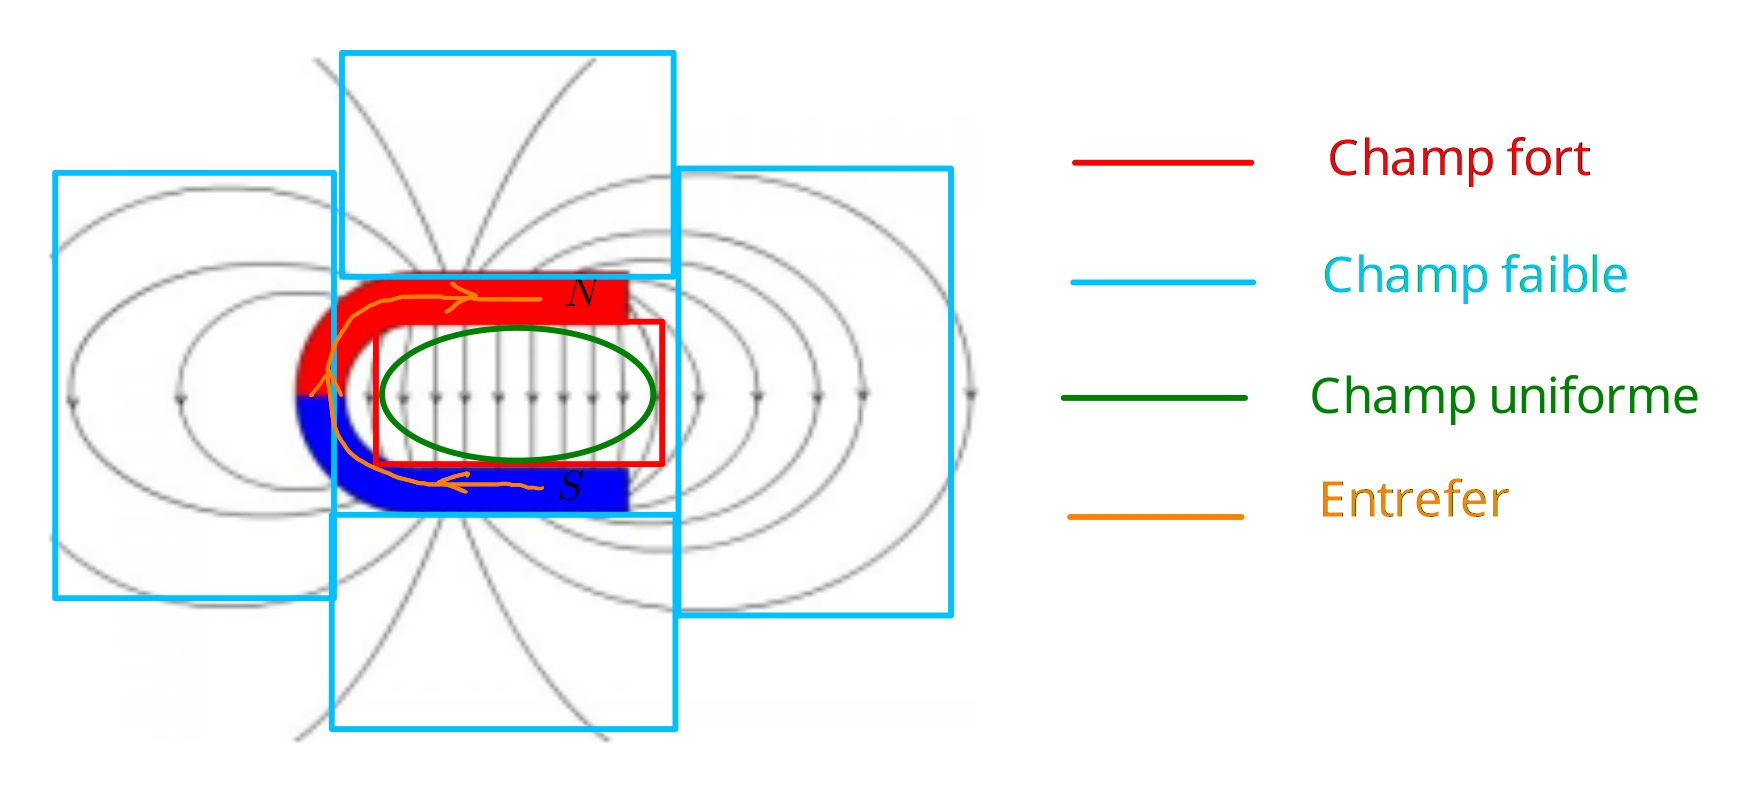
\includegraphics[width=\linewidth]{exaimu_corr}
    \captionof{figure}{Correction aimant en U.}
    \label{fig:exaimucorr}
  \end{center}
\end{minipage}

\section{Cartes de champ}
\label{sec:excchp}
Voir Figure~\ref{fig:excchpcorr}.
\begin{itemize}[label=$\diamond$, leftmargin=10pt]
  \item Le champ est le plus intense là où les LdC sont très rapprochées, et
    faible là où il y a peu de LdC.
  \item Les LdC s'enroulent autour des sources, qui sont donc situées au niveau
    des points noirs de chaque figure. Il y en a six sur la figure de gauche, et
    4 sur la figure de droite. Comme on nous indique que ce sont des spires, on
    a \textbf{3 spires} à gauche et \textbf{2 spires} à droite.
  \item Connaissant l'enroulement des LdC, le sens du courant dans les fils se
    déduit de la règle de la main droite (l'enroulement des doigts donne le sens
    des LdC, le pouce donne le sens du courant). Dans tous les cas, le courant
    est perpendiculaire au plan de la feuille.
    \smallbreak
    Sur la carte de gauche, le courant sort du plan de la feuille $\odot$ pour
    les 3 sources de gauche, et rentrent dans le plan de la feuille $\otimes$
    pour les 3 sources de droite.
    \smallbreak
    Sur la carte de droite, le courant sort du plan de la feuille $\odot$ en haut à
    droite et en bas à gauche, et rentre $\otimes$ en haut à gauche et en bas à
    droite.
\end{itemize}

\begin{figure}[h]
  \centering
  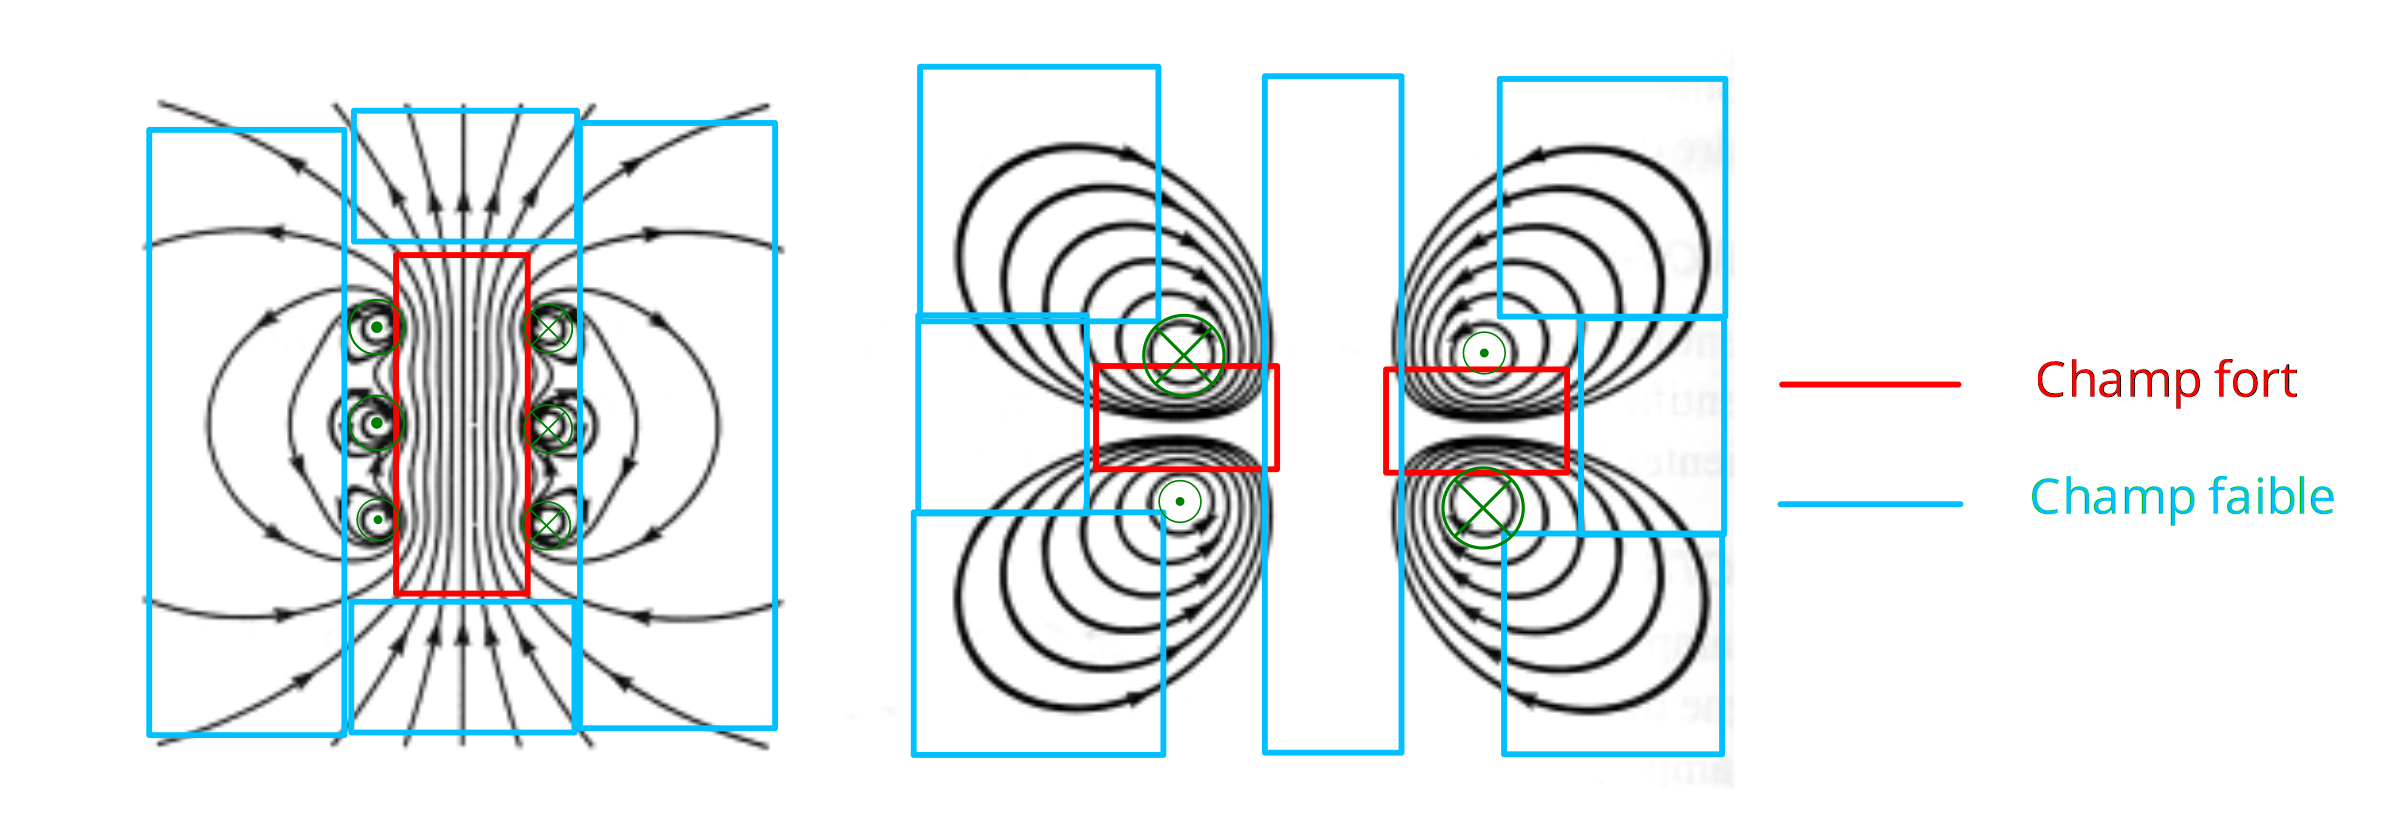
\includegraphics[width=\linewidth]{cchp_corr}
  \caption{Correction cartes de champ.}
  \label{fig:excchpcorr}
\end{figure}

\section{Aimantation d'un matériau}
\label{sec:aimat}
\begin{enumerate}
  \item Le moment magnétique d'une spire plane d'aide $S$ et parcourue par un
    courant $I$ a pour norme $\norm{\vv{\mu}} = SI$. On en déduit qu'un moment
    magnétique s'exprime en \si{A.m^2}. En divisant par un volume en \si{m^3},
    on obtient bien des \si{A.m^{-1}}.
  \item Un aimant est d'autant meilleur que son moment magnétique est élevé et
    son volume faible~: un bon aimant doit donc être fait d'un matériau qui
    possède une \textbf{forte aimantation}.
  \item Pour une aimantation $M = \SI{3e6}{A.m ^{-1}}$, le moment magnétique de
    l'aimant en question vaut
    \[
      \boxed{\mu_{\rm aimant} = M\times\pi R^2 e = \SI{0.2}{A.m^2}}
    \]
  \item Le moment magnétique d'un ensemble de $N$ spires juxtaposées montées en
    série vaut $\mu_{\rm spires} = NI\pi R^2$. Pour avoir le même moment que l'aimant
    précédent, on doit avoir
    \[
      \mu_{\rm aimant} = \mu_{\rm spires}
      \Lra 
      M\pi R^2 e = NI\pi R^2
      \qso
      \boxed{N = \frac{Me}{I} = \num{3e4}}
    \]
    c'est-à-dire \num{30000} spires~! On retiendra qualitativement que le
    magnétisme de la matière est bien plus fort que le magnétisme des courants.
\end{enumerate}

\section{Équilibre d'un aimant}
\label{sec:exeqaim}
\noindent
\begin{minipage}[t]{.7\linewidth}
  Un aimant très fin, de moment magnétique $\vv{\mu}$ et de masse $m$, repose en
  équilibre sur une pointe en O. Il est soumis à l'action d'un champ magnétique
  uniforme $\vv{B}$ et au champ de pesanteur terrestre $\vv{g}$. On appelle G le
  centre d'inertie de l'aimant.
  \smallbreak
  Exprimer la distance $d = \rm OG$ pour que l'aimant reste en équilibre
  horizontal.
\end{minipage}
\hfill
\begin{minipage}[t]{.3\linewidth}
  ~
  \vspace*{-20pt}
  \begin{center}
    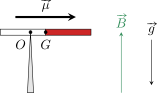
\includegraphics[scale=1]{exeqaim}
    \label{fig:exeqaim}
  \end{center}
\end{minipage}

\section{Rails de \textsc{Laplace} inclinés}
\label{sec:railpl}
On reprend les rails de \textsc{Laplace}, mais en les inclinant~: au lieu d'être
horizontaux, ils forment un angle $\alpha = \ang{30;;}$ avec la verticale. Le
champ magnétique est supposé stationnaire, uniforme, vertical dirigé vers le
haut, de norme \SI{150}{mT}. Le barreau mobile des rails de \textsc{Laplace}
pèse \SI{8.0}{kg} et est long de $\ell = \SI{12}{cm}$. Les frottements sont
négligés, de même que tout phénomène d'induction.
\begin{enumerate}
  \item Faire un schéma du dispositif en représentant les différentes forces
    agissant sur le barreau mobile. Quel doit être le sens du courant dans le
    circuit pour que la force de \textsc{Laplace} retienne le barreau~?
  \item Déterminer l'intensité du courant permettant l'équilibre du barreau.
  \item Partant de cette situation, on communique au barreau une vitesse
    initiale $v_0$ dirigée vers le haut. Déterminer son mouvement ultérieur.
  \item En raisonnant à partir de la loi de \textsc{Lenz} (chapitre suivant),
    indiquer qualitativement comment est modifiée la réponse à la question
    précédente lorsque l'on tient compte de l'induction.
\end{enumerate}

\section{Mesure du champ magnétique terrestre}
\label{sec:meschpterre}
Dans un laboratoire situé à Paris, on souhaite déterminer la norme
$\norm{\vv{B}_h}$ de la composante horizontale locale $\vv{B}_h$ (dont le sens
et la direction sont donnés sur la Figure~\ref{fig:magTsens}) grâce à un
dispositif d'\textsc{Œrsted} (Figure~\ref{fig:orsted}). Ce dernier est constitué
d'une aiguille aimantée libre de pivoter sans frottement sur son axe, fixé à un
socle transparent et un fil de cuivre relié à deux bornes de sécurité fixées au
même socle transparent, de courant admissible \SI{5}{A}.
\noindent
\begin{minipage}[t]{.5\linewidth}
  \begin{center}
    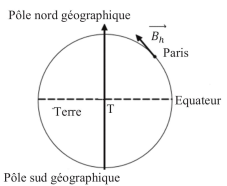
\includegraphics[scale=1]{magTsens}
    \captionof{figure}{Sens de la composante horizontale locale du champ
    magnétique terrestre à Taris.}
    \label{fig:magTsens}
  \end{center}
\end{minipage}
\hfill
\begin{minipage}[t]{.5\linewidth}
  \begin{center}
    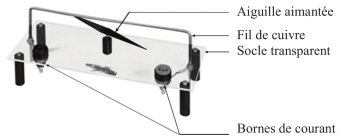
\includegraphics[scale=1]{orsted}
    \captionof{figure}{Dispositif d'\textsc{Œrsted}}
    \label{fig:orsted}
  \end{center}
\end{minipage}
\begin{rexem}{Matériel}
  \noindent
  \begin{minipage}[t]{.5\linewidth}
    \begin{itemize}[label=$\diamond$, leftmargin=10pt]
      \item un rapporteur~;
      \item des files électriques~;
      \item un interrupteur~;
    \end{itemize}
  \end{minipage}
  \hfill
  \begin{minipage}[t]{.5\linewidth}
    \begin{itemize}[label=$\diamond$, leftmargin=10pt]
      \item une alimentation électrique stabilisée \SIrange{0}{30}{V}/\SI{5}{A}~;
      \item un ampèremètre~;
      \item un teslamètre permettant la mesure d'intensité de champs
        magnétiques entre \SIrange{0.1}{100}{mT}.
    \end{itemize}
  \end{minipage}
\end{rexem}
\begin{tdefi}{Donnée}
  Le champ magnétique créé par un fil infini parcouru par un courant $I$
  s'exprime, dans un système de coordonnées cylindriques d'axe $z$ orienté par
  le sens réel du courant, par~:
  \[
    \vv{B} = \frac{\mu_0 I}{2\pi r}\ut
  \]
  avec $\mu_0 = 4\pi \cdot \SI{e-7}{H.m^{-1}}$. On admet que le champ créé par
  le fil du dispositif d'\textsc{Œrsted} est convenablement décrit par cette
  expression.
\end{tdefi}
On souhaite établir un protocole permettant de mesurer la composante horizontale
locale du champ magnétique terrestre à Paris en exploitant le principe de
superposition des champs magnétiques.
\begin{enumerate}
  \item Pour quelle raison ne peut-on pas se servir directement du teslamètre
    pour effectuer la mesure~?
  \item On suppose que le fil est parcouru par un courant d'intensité $I =
    \SI{1}{A}$. Calculer la valeur du champ magnétique à $r = \SI{2}{cm}$ du
    fil.
  \item Décrire et schématiser l'expérience à réaliser en vous servant du
    matériel mis à votre disposition, exception faite du teslamètre.
  \item Préciser les mesures à réaliser, et la technique numérique à employer
    pour trouver la valeur.
  \item Donner un ordre de grandeur des grandeurs physiques à employer pour
    réaliser l'expérience.
\end{enumerate}

\end{document}
